\newpage
\section{Ôn tập chương 6}
\def\thoigian{90}%--Thời gian
\de{Đề số 1}{Chương VI. Thống kê}

\begin{center}
	\textbf{PHẦN 1 - CÂU TRẮC NGHIỆM BỐN PHƯƠNG ÁN}
\end{center}
\Opensolutionfile{ans}[ans/ans-TN-0D6-DE1]
\begin{ex}%[0D6N1-4]%[Dự án D - đợt 2 NH24-25- Lâm Chính]
	Khi sử dụng máy tính bỏ túi với $10$ chữ số thập phân ta được $\sqrt{11}=3{,}31662479$. Giá trị gần đúng của $\sqrt{11}$ chính xác đến hàng phần nghìn là
	\choice
	{$3{,}316$}
	{\True $3{,}317$}
	{$3{,}31$}
	{$3{,}318$}
	\loigiai{
		Giá trị gần đúng của $\sqrt{11}=3{,}31662479$ chính xác đến hàng phần nghìn là $3{,}317$.
	}
\end{ex}
\begin{ex}%[0D6N1-3]%[Dự án D - đợt 2 NH24-25- Lâm Chính]
	Quy tròn số $8\,386{,}675796$ đến chữ số hàng phần trăm ta được số gần đúng là
	\choice
	{$8400$}
	{\True $8386{,}68$}
	{$8386{,}676$}
	{$8386{,}67$}
	\loigiai{
		Số quy tròn của số $8\,386{,}675796$ đến hàng phần trăm là $8\,386{,}68$.}
\end{ex}
\begin{ex}%[0D6H1-1]%[Dự án D - đợt 2 NH24-25- Lâm Chính]
	Bác nông dân đo mảnh vườn hình chữ nhật có chiều dài $ 5\pm0{,}03 $ m và chiều rộng $ 3\pm0{,}01 $ m. Xác định sai số tương đối của phép đo diện tích mảnh vườn.
	\choice
	{$ 0{,}75\% $}
	{$ 0{,}85\% $}
	{\True $ 0{,}95\% $}
	{$ 0{,}1\% $}
	\loigiai{
		Gọi $ x $, $ y $ là chiều dài và chiều rộng của vườn.\\
		Ta có $ \heva{&x=5\pm0{,}03\text{ m}\\ &y=3\pm0{,}01\text{ m}} \Rightarrow \heva{&4{,}97\leq x\leq5{,}03\\ &2{,}99\leq y\leq3{,}01.} $\\
		Gọi diện tích mảnh vườn là S, khi đó $ 14{,}8603\leq S\leq15{,}1403 \Rightarrow S=14{,}72\pm0{,}14 $ m$ ^2 $.\\
		Vậy sai số tương đối trong phép đo là $ \delta\leq\dfrac{0{,}14}{14{,}72} \approx0{,}0095=0{,}95\% $.
	}
\end{ex}
%%%
\begin{ex}%[0D6H2-1]%[Dự án D - đợt 2 NH24-25- Lâm Chính]
	Trong $6$ tháng đầu năm, số sản phẩm bán ra mỗi tháng của một của hàng đều tăng khoảng $20 \%$ so với tháng trước đó. Biết rằng, trong bảng dưới đây, số sản phẩm bán ra của một tháng bị nhập sai. Hãy tìm tháng đó.
	\begin{center}
		\begin{tabular}{|c|c|c|c|c|c|c|}
			\hline Tháng & $1$ & $2$ & $3$ & $4$ & $5$ & $6$ \\
			\hline Số sản phẩm bán ra & $145$ & $175$ & $211$ & $256$ & $340$ & $371$ \\
			\hline
		\end{tabular}
	\end{center}
	\choice
	{Tháng $3$}
	{Tháng $4$}
	{\True Tháng $5$}
	{Tháng $6$}
	\loigiai{Tỉ lệ phần trăm tăng thêm của số sản phẩm bán ra của tháng thứ $2$ so với tháng $1$ được tính như sau $$\dfrac{175-145}{145} \times 100=\dfrac{600}{29} \approx 20{,}7 \%.$$
		Với cách tính như trên, tỉ lệ phần trăm tăng thêm của số sản phẩm bán ra mỗi tháng được tính ở bảng dưới đây
		\begin{center}
			\begin{tabular}{|c|c|c|c|c|c|}
				\hline Tháng & $2$ & $3$ & $4$ & $5$ & $6$ \\
				\hline Tỉ lệ phần trăm tăng thêm so với tháng trước & $20{,}7 \%$ & $20{,}6 \%$ & $21{,}3 \%$ & $32{,}8 \%$ & $9{,}1 \%$ \\
				\hline
			\end{tabular}	
		\end{center}
		Ta thấy tỉ lệ tăng của tháng $5$ và tháng $6$ đều khác xa với $20 \%$. Do đó trong bảng số liệu đã cho, số sản phẩm của tháng $5$ là không chính xác.}
\end{ex}
\begin{ex}%[0D6H2-2]%[Dự án D - đợt 2 NH24-25- Lâm Chính]
	Biểu đồ hình bên cho biết thông tin về kết quả học lực của học sinh khối $10$ của một trường THPT như sau
	\begin{center}
		\begin{tikzpicture}[
			line join = round, line cap = round,
			declare function={x=2; y=2; kcy=1.5; kc=3.0; dochia=20; },
			xscale = 1/x, yscale = 1/y, 
			font = \scriptsize]
			\foreach \x/\y[count = \i from 0] in {Giỏi/38,Khá/140,Trung bình/52,Yếu/13}{
				\pgfmathsetmacro{\j}{kcy + (kc+1)*\i}
				\draw[pattern = north east lines] (\j-.5,0) rectangle (\j+.5,\y/dochia);
				\path (\j,\y/dochia) node[above]{$\y$};
				\path (\j,-.5*y) node[]{\x};
				\global\let\n=\j}
			\draw (\n+x,0) -| (-.5,160/dochia+y/dochia);
			\foreach \y in {0,20,40,60,80,100,120,140,160}{
				\draw (-.5+.05*x,\y/dochia)--(-.5-.05*x,\y/dochia) node[left]{$\y$};
				\draw [gray!50] (-0.5,\y/dochia)--(\n+x,\y/dochia);}
			\path (current bounding box.north) node[above]{\bf\large Xếp loại học lực học sinh khối 10};
			\draw[blue, rounded corners = 8pt, thick] (current bounding box.south west) rectangle (current bounding box.north east);
		\end{tikzpicture}
	\end{center}
	Phát biểu nào sau là \textbf{sai}?
	\choice
	{Số học sinh của khối $10$ là $243$ học sinh}
	{Số học sinh khá lớn hơn tổng số học sinh giỏi, trung bình và yếu}
	{\True Số học sinh khá gấp $5$ lần số học sinh giỏi}
	{Số học sinh trung bình gấp $4$ lần số học sinh yếu}

	\loigiai{
		\begin{itemize}
			\item Số học sinh của khối $10$ là $38+140+52+13=243$ (học sinh).
			\item Tổng số học sinh giỏi, trung bình và yếu bằng $38+52+13=103 < 140$ nên số học sinh khá lớn hơn tổng số học sinh giỏi, trung bình và yếu. 
			\item Tỉ số giữa số học sinh khá và số học sinh giỏi là $\dfrac{140}{38} \approx 3{,}7$. Do đó \lq\lq Số học sinh khá gấp $5$ lần số học sinh giỏi\rq\rq~ là phát biểu sai.
			\item Số học sinh trung bình gấp $4$ lần số học sinh yếu.
		\end{itemize}
	}
\end{ex}
\begin{ex}%[0D6H2-2]%[Dự án D - đợt 2 NH24-25- Lâm Chính]
	Sản lượng nuôi tôm phân theo địa phương của các tỉnh Cà Mau và Tiền Giang được thể hiện ở hai biểu đồ sau (đơn vị: tấn)
	\begin{center}
		\begin{tikzpicture}[>=stealth,line join=round,line cap=round,font=\footnotesize,yscale=0.22,scale=0.5]
			\begin{scope}
				\def\h{30};
				\def\a{10};
				\draw[black!20] (0,{\h+2})node[right=2cm,black]{Cà Mau}--(0,0)--(1.5,0) node[below,black]{\tiny Năm $2008$}--(4.5,0) node[below,black]{\tiny Năm $2013$}--(7.5,0) node[below,black]{\tiny Năm $2018$}--(\a,0);
				\foreach \y/\z in {
					0/75000,
					5/100000,
					10/125000,
					15/150000,
					20/175000,
					25/200000
				} 
				\draw[black!20] (0,\y) node[left=2mm,black]{\tiny $\z$}--(\a,\y);
				\foreach \x/\y in {1/4,4/14,7/25.5}{
					\draw[fill=cyan] (\x,0) rectangle (\x+1,\y);
				}
			\end{scope}
			\begin{scope}[shift={(13,0)}]
				\def\h{30};
				\def\a{10};
				\draw[black!20] (0,{\h+2})node[right=2cm,black]{Tiền Giang}--(0,0)--(1.5,0) node[below,black]{\tiny Năm $2008$}--(4.5,0) node[below,black]{\tiny Năm $2013$}--(7.5,0) node[below,black]{\tiny Năm $2018$}--(\a,0);
				\foreach \y/\z in {
					0/0,
					5/5000,
					10/10000,
					15/15000,
					20/20000,
					25/25000,
					30/30000
				} 
				\draw[black!20] (0,\y) node[left=2mm,black]{\tiny $\z$}--(\a,\y);
				\foreach \x/\y in {1/10,4/17.5,7/29}{
					\draw[fill=cyan] (\x,0) rectangle (\x+1,\y);
				}
			\end{scope}
			\path (10,-5.5)node{(Nguồn: Tổng cục Thống kê)};
		\end{tikzpicture}
	\end{center}
	Phát biểu nào sau là đúng?
	\choice
	{Sản lượng nuôi tôm mỗi năm của tỉnh Tiền Giang đều cao hơn tỉnh Cà Mau}
	{Ở tỉnh Cà Mau, sản lượng nuôi tôm năm $2018$ tăng gấp hơn $4$ lần so với năm $2008$}
	{\True Ở tỉnh Tiền Giang, sản lượng nuôi tôm năm $2018$ tăng gấp hơn $2{,}5$ lần so với năm $2008$}
	{Ở tỉnh Tiền Giang, từ năm $2008$ đến năm $2018$, sản lượng nuôi tôm mỗi năm tăng trên $50 \%$ so với năm cũ}
	\loigiai{
		\begin{itemize}
			\item Sản lượng nuôi tôm năm $2018$ của tỉnh Tiền Giang thấp hơn tỉnh Cà Mau.
			\item Ở tỉnh Cà Mau, sản lượng nuôi tôm năm $2018$ tăng xấp xỉ gấp hơn $2$ lần so với năm $2008$.
			\item Ở tỉnh Tiền Giang, sản lượng nuôi tôm năm $2018$ tăng gấp hơn $2{,}5$ lần so với năm $2008$.
			\item Ở tỉnh Tiền Giang vào năm $2018$, sản lượng nuôi tôm mỗi năm tăng dưới $50 \%$ so với năm cũ.
		\end{itemize}
	}
\end{ex} 
\begin{ex}%[0D6N4-2]%[Dự án D - đợt 2 NH24-25- Lâm Chính]
	\immini{Biểu đồ đoạn thẳng ở hình bên biểu diễn giá vàng bán ra trong bảy ngày đầu tiên của tháng $6$ năm $2021$. Tìm khoảng biến thiên của mẫu số liệu.
	}
	{\color{blue} 
		\begin{tikzpicture}[scale=0.8, font=\footnotesize, line join=round, line cap=round, >=stealth]	
			\draw[->,>=stealth,line width=1.5] (0,0)--(0,6); \draw[->,>=stealth,line width=1.5] (0,0)--(8.5,0);
			\draw 
			(-0.6,0) node {$5 710$}
			(-0.6,1.1) node {$5 722$}
			(-0.6,1.5) node {$5 727$}
			(-0.6,2.5) node {$5737$}
			(-0.6,3.5) node {$5747$}
			(-0.6,4.5) node {$5757$}
			(-0.6,5.5) node {$5767$}
			(0,6.4) node {Giá vàng (nghìn đồng/chỉ)}
			
			(1,-0.5) node {$1/6$}
			(2,-0.5) node {$2/6$}
			(3,-0.5) node {$3/6$}
			(4,-0.5) node {$4/6$}
			(5,-0.5) node {$5/6$}
			(6,-0.5) node {$6/6$}
			(7,-0.5) node {$7/6$}
			(8.2,-0.5) node {Ngày};
			
			\draw[line width=1.5,red] (1,5.5)--(2,4.5)--(3,2.5)--(4,1.5)--(5,3.5)--(6,3.5)--(7,1.2);
			\draw[dashed] (0,5.5)--(1,5.5)--(1,0) (0,4.5)--(2,4.5)--(2,0) (0,2.5)--(3,2.5)--(3,0) (0,1.5)--(4,1.5)--(4,0) (0,3.5)--(5,3.5)--(5,0) (6,3.5)--(6,0) (0,1.2)--(7,1.2)--(7,0);
			\fill[black] (1,5.5) circle (2.5pt);
			\fill[black] (2,4.5)circle (2.5pt);
			\fill[black] (3,2.5)circle (2.5pt);
			\fill[black] (4,1.5)circle (2.5pt);
			\fill[black] (5,3.5)circle (2.5pt);
			\fill[black] (6,3.5)circle (2.5pt);
			\fill[black] (7,1.2) circle (2.5pt);
		\end{tikzpicture}
	}
	%\begin{flushright}
	%\textit{Nguồn https://bieudogiavang.vn\\
		%{\color{blue} Hình 4}}
	%\end{flushright}
	\choice 
	{$41$}
	{$43$}
	{\True $45$}
	{$47$}
	\loigiai{
		\begin{itemize}
			\item 	Mẫu số liệu thống kê tốc độ tăng trưởng GDP nhận được
			\begin{center}
				\begin{tabular}{|c|c|c|c|c|c|c|c|}
					\hline
					Ngày & $1/6$ & $2/6$ & $3/6$ & $4/6$ & $5/6$ & $6/6$ & $7/6$ \\
					\hline
					Giá vàng (nghìn đồng/chỉ) & $5767$ & $5757$ & $5737$ & $5727$ & $5747$ & $5747$ & $5722$ \\
					\hline
				\end{tabular}\\
				Sắp xếp lại mẫu số liệu theo thứ tự không giảm
				\begin{center}
					\begin{tabular}{cccccccc}
						&	$5722$ & $5727$ & $5737$ & $5747$& $5747$ & $5757$ & $5767$  \\
					\end{tabular}
				\end{center}
			\end{center}
			\item Khoảng biến thiên của mẫu số liệu là $R=5767-5722=45$.
		\end{itemize}
	}
\end{ex}
\begin{ex}%[0D6N4-1]%[Dự án D - đợt 2 NH24-25- Lâm Chính]
	Số đặc trưng nào sau đây đo độ phân tán của mẫu số liệu?
	\choice
	{Trung vị}
	{Mốt}
	{Số trung bình}
	{\True Độ lệch chuẩn}
	\loigiai{
		Số đặc trưng đo độ phân tán của mẫu số liệu là độ lệch chuẩn.
	}
\end{ex}
\begin{ex}%[0D6H3-5]%[Dự án D - đợt 2 NH24-25- Lâm Chính]
	Một bác sĩ mắt ghi lại tuổi của $30$ bệnh nhân mắc bệnh đau mắt hột. Kết quả thu được mẫu số liệu như sau
	\begin{center}
		\begin{tabular}{|p{0.5cm}p{0.5cm}p{0.5cm}p{0.5cm}p{0.5cm}p{0.5cm}p{0.5cm}p{0.5cm}p{0.5cm}p{0.5cm}|}
			\hline
			$21$    & $17 $   & $22 $   & $18 $   & $20$    & $17$    & $15$    & $13$    & $15$    & $20$ \\
			$15$    & $12$    & $18 $   & $17$    & $25$    & $17$    & $21 $   & $15$    & $12$    & $18$ \\
			$16 $   & $23 $   & $14 $   & $18$    & $19$    & $13$    & $16$    & $19$    & $18$    & $17$ \\
			\hline
		\end{tabular}
	\end{center}
	Tính mốt của bảng số liệu đã cho. 
	\choice
	{\True $17$ và $18$}
	{$25$ và $16$}
	{$16$ và $17$}
	{$25$ và $18$}
	\loigiai{
		Từ bảng số liệu trên ta suy ra bảng phân bố tần số tuổi của $30$ bệnh nhân đau mắt hột như sau
		\begin{center}
			\begin{tabular}{|c|c|c|c|c|c|c|c|c|c|c|c|c|c|c|}
				\hline    
				Tuổi  & $12$    & $13$    & $14$    & $15$    & $16$    & $17$    & $18$    & $19$    & $20$    & $21$    & $22$    & $23$    & $25$    & Tổng \\
				\hline    
				Số bệnh nhân & $2$     & $2$     & $1$     & $4$     & $2$     & $5$     & $5$     & $2$     & $2$     & $2$     & $1$     & $1$     & $1$     & $30$ \\
				\hline   
			\end{tabular}
		\end{center}
		Ta thấy tuổi $17$ và $18$ có tần số bằng $5$ là lớn nhất. Do đó bảng số liệu có hai mốt là $17$ và $18$.
	}
\end{ex}
\begin{ex}%[0D6H3-4]%[Dự án D - đợt 2 NH24-25- Lâm Chính]
	Số điểm của $5$ vận động viên bóng rổ được ghi trong trận đấu như sau:
	\begin{center}
		\begin{tabular}{ccccc}
			$9$& $8$& $15$& $8$& $20$.
		\end{tabular}
	\end{center}
	Tứ phân vị thứ nhất của mẫu số liệu trên là
	\choice
	{\True $Q_1=8$}
	{$Q_1=8{,}5$}
	{$Q_1=9$}
	{$Q_1=20$}
	\loigiai{
		Sắp xếp các giá trị theo thứ tự không giảm
		\begin{center}
			\begin{tabular}{ccccc}
				$8$& $8$& $9$& $15$& $20$
			\end{tabular}
		\end{center}
		Vì $n=5$ là số lẻ nên $Q_2$ là giá trị chính giữa. Do đó $Q_2=9$.\\
		Ta có $Q_1$ là trung vị của nửa số liệu bên trái. Suy ra  $Q_1=\dfrac{8+8}{2}=8$.
	}
\end{ex}
\begin{ex}%[0D6H4-4]%[Dự án D - đợt 2 NH24-25- Lâm Chính]
	Tốc độ tăng trưởng GDP của Việt Nam giai đoạn 2014 $-$ 2021 được biểu diễn trong hình vẽ bên dưới. Độ lệch chuẩn của mẫu số liệu là
		\choice
		{\True $1{,}72$}
		{$1{,}77$}
		{$1{,}81$}
		{$1{,}64$}
		\begin{center}
			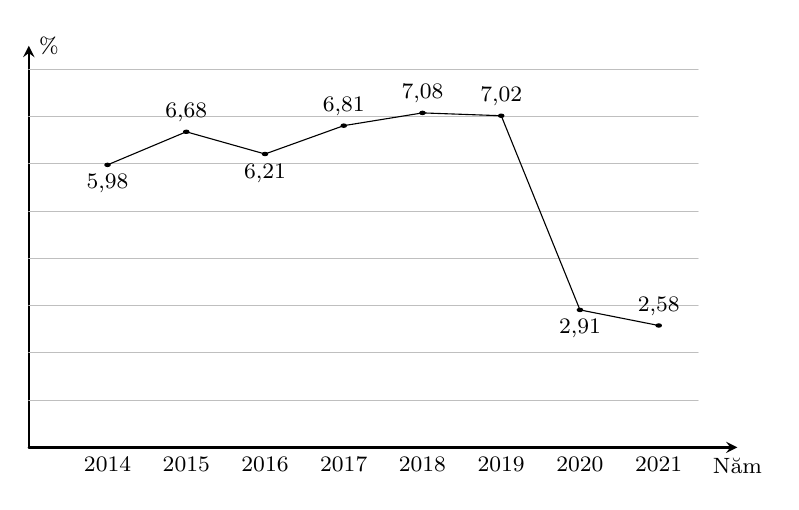
\begin{tikzpicture}[>=stealth,line join=round,line cap=round,font=\footnotesize,yscale=0.6]
			\draw [->,thick] (0,0)--(9,0) node[below]{Năm};
			\draw [->,thick] (0,0)--(0,8.5) node[right]{$\%$};
			\foreach \x in {1,2,3,4,5,6,7,8}
			\draw[gray!50] (0,\x)--(8.5,\x) ;
			\draw[fill] 
			(1,5.98) circle (1pt) node[below]{$5{,}98$} (1,0) node[below]{$2014$}
			(2,6.68) circle (1pt) node[above]{$6{,}68$} (2,0) node[below]{$2015$}
			(3,6.21) circle (1pt) node[below]{$6{,}21$} (3,0) node[below]{$2016$}
			(4,6.81) circle (1pt) node[above]{$6{,}81$} (4,0) node[below]{$2017$}
			(5,7.08) circle (1pt) node[above]{$7{,}08$} (5,0) node[below]{$2018$}
			(6,7.02) circle (1pt) node[above]{$7{,}02$} (6,0) node[below]{$2019$}
			(7,2.91) circle (1pt) node[below]{$2{,}91$} (7,0) node[below]{$2020$}
			(8,2.58) circle (1pt) node[above]{$2{,}58$} (8,0) node[below]{$2021$}
			; 
			\draw (1,5.98)--(2,6.68)--(3,6.21)--(4,6.81)--(5,7.08)--(6,7.02)--(7,2.91)--(8,2.58); 
		\end{tikzpicture}
		\end{center}
	\loigiai{
		Số trung bình là 
		\[
		\overline{x} = \dfrac{5{,}98+6{,}68+6{,}21+6{,}81+7{,}08+7{,}02+2{,}91+2{,}58}{8} = 5{,}65875.  
		\]
		Phương sai của mẫu số liệu 
		\begin{align*}
			s^2 &= \dfrac{1}{8} \left( 5{,}98-\overline{x}\right)^2 + \left(6{,}68-\overline{x}\right)^2 + \left(6{,}21-\overline{x}\right)^2+ \left(6{,}81-\overline{x}\right)^2 \\
			&+ \left(7{,}08-\overline{x}\right)^2 + \left(7{,}02-\overline{x}\right)^2 + \left(2{,}91-\overline{x}\right)^2+ \left(2{,}58-\overline{x}\right)^2 \Big) \\
			&\approx 2{,}96. 
		\end{align*}
		Độ lệch chuẩn của mẫu số liệu là $s \approx 1{,}72$.
	}
\end{ex}
\begin{ex}%[0D6H4-3]%[Dự án D - đợt 2 NH24-25- Lâm Chính]
	Điểm thi HK2 môn Toán của một lớp $30$ học sinh như sau:
	\begin{center}
		\begin{tabular}{|c|c|c|c|c|c|c|c|c|c|c|c|c|c|c|}
			\hline 
			4 & 5 & 3 & 5 & 9 & 5{,}5 & 6 & 7 & 10 & 9 & 5 & 6{,}5 & 7 & 8 & 6 \\ 
			\hline 
			7 & 9 & 8 & 5 & 7{,}5 & 8 & 6 & 2 & 9 & 7 & 6 & 5{,}5 & 5 & 6 & 7 \\ 
			\hline 
		\end{tabular} 
	\end{center}
	Có bao nhiêu giá trị ngoại lệ trong mẫu số liệu đã cho?
	\choice
	{\True $0$}
	{$1$}
	{$2$}
	{$3$}
	\loigiai{
		Từ mẫu số liệu đã cho  ta tính được $Q_1= 5$;  $Q_3= 8$. \\
		Khoảng tứ phân vị là $\Delta_Q = 8-5 =3$.  \\
		Ta có $Q_1 - \dfrac{3}{2}\Delta_Q = 0{,}5$;  $Q_3 + \dfrac{3}{2}\Delta_Q = 12{,}5$.   \\
		Vậy không có giá trị ngoại lệ trong mẫu số liệu.
	}
\end{ex}
\Closesolutionfile{ans}
%\begin{center}
%	\textbf{ĐÁP ÁN}
%	\inputansbox{10}{ans/ans-TN-0D6-DE1}	
%\end{center}

\begin{center}
	\textbf{PHẦN 2 - CÂU TRẮC NGHIỆM ĐÚNG SAI}
\end{center}
\setcounter{ex}{0}
\Opensolutionfile{ans}[ans/ans-DS-0D6-DE1]
\begin{ex}%[0D6H4-4]%[Dự án D - đợt 2 NH24-25- Lâm Chính]
	Điều tra thu nhập của $40$ hộ gia đình ở một bản được số liệu như sau
	\begin{center}
		\begin{tabular}{|c|c|c|c|c|c|c|c|c|c|}
			\hline Thu nhập (triệu đồng/năm) & $4$ & $4{,}5$ & $5$ & $5{,}5$ & $6$ & $6{,}5$ & $7$ & $7{,}5$ & $8$  \\
			\hline Số hộ gia đình & $1$ & $3$ & $4$ & $6$ & $8$ & $7$ & $6$ & $3$ & $2$ \\
			\hline 
		\end{tabular}
	\end{center}
	\choiceTF
	{\True Cỡ mẫu là $40$}
	{Mốt của mẫu số liệu là $8$}
	{\True Số trung bình của mẫu số liệu trên là $6{,}1125$}
	{Phương sai của mẫu số liệu trên là $1{,}956$ (kết quả làm tròn đến hàng phần nghìn)}
	\loigiai{
		\begin{itemchoice}
			\itemch Từ giả thiết ta có cỡ mẫu là $40$.
			\itemch Có $8$ hộ gia đình thu nhập $6$ triệu đồng/năm nên mốt là $6$.
			\itemch Số trung bình của mẫu số liệu trên là \[\overline{x}=\dfrac{4\cdot 1+4{,}5\cdot 3+5\cdot 4+5{,}5\cdot 6+6\cdot 8+6{,}5\cdot 7+7\cdot 6+7{,}5\cdot 3 +8\cdot 2}{40}=6{,}1125.\]
			\itemch Phương sai của mẫu số liệu trên là 
			\begin{align*}
				s^2 &= \dfrac{1}{40}\left(4^2\cdot 1+4{,}5^2\cdot 3+5^2\cdot 4+5{,}5^2\cdot 6+6^2\cdot 8+6{,}5^2\cdot 7+7^2\cdot 6+7{,}5^2\cdot 3 +8^2\cdot 2\right)-6{,}1125^2
				\\ &\approx 0{,}9561.
			\end{align*}
		\end{itemchoice}
	}
\end{ex}
\begin{ex} %[0D6H4-4]%[Dự án D - đợt 2 NH24-25- Lâm Chính]
	Cho mẫu số liệu về chiều cao đầu năm học của một nhóm học sinh lớp $10$ như sau  
	\begin{center}
		\begin{tabular}{|l|c|c|c|c|c|}
			\hline
			Chiều cao (cm) & $150$ & $155$ & $160$ & $165$ & $170$ \\
			\hline
			Tần số & $25$ & $28$ & $103$ & $44$ & $13$ \\
			\hline
		\end{tabular}
	\end{center}
	Khi đó 
	\choiceTF 
	{Tìm khoảng biến thiên của mẫu số liệu là $R=10$} 
	{\True Tứ phân vị thứ nhất là $Q_1=157{,}5$} 
	{\True Số trung bình cộng của mẫu số liệu là $\overline{x}=159{,}8$ (làm tròn kết quả đến hàng phần chục)} 
	{\True Độ lệch chuẩn của mẫu số liệu là $S=5{,}492$ (làm tròn kết quả đến hàng phần nghìn)}  
	\loigiai{
		\begin{itemchoice} 
			\itemch 
			Khoảng biến thiên của mẫu số liệu $R=170-150=20$.  
			\itemch 
			Tứ phân vị thứ nhất $Q_1=\dfrac{155+160}{2}=157{,}5$.  
			\itemch
			Số trung bình cộng của mẫu số liệu là \\ 
			$\overline{x}=\dfrac{150 \cdot 25 + 155 \cdot 28 + 160 \cdot 103 + 165 \cdot 44 + 170 \cdot 13}{25+28+103+44+13}=159{,}8$.  
			\itemch
			Phương sai của mẫu số liệu \\ 
			$S^2=\dfrac{1}{213}\left(150^2 \cdot 25 + 155^2 \cdot 28 + 160^2 \cdot 103 + 165^2 \cdot 44 + 170^2 \cdot 13 \right) - (\overline{x})^2=30,16$. \\ 
			Độ lệch chuẩn là $S=\sqrt{S^2}=5{,}492$.  
		\end{itemchoice}  
	}
\end{ex}
\Closesolutionfile{ans}
%\inputansbox[2]{2}{ans/ans-DS-0D6-DE1}



\begin{center}
	\textbf{PHẦN 3 - CÂU TRẮC NGHIỆM TRẢ LỜI NGẮN}
\end{center}
\setcounter{ex}{0}
\Opensolutionfile{ans}[ans/ans-KQ-0D6-DE1]

\begin{ex}%[0D6H1-2]%[Dự án D - đợt 2 NH24-25- Lâm Chính]
	Một sân bóng đá có dạng hình chữ nhật với chiều dài và chiều rộng của sân lần lượt là $105$ m và $68$ m. Khoảng cách xa nhất giữa hai vị trí trên sân đúng bằng độ dài đường chéo của sân. Quy tròn giá trị gần đúng (theo đơn vị mét) của độ dài đường chéo sân đến hàng phần mười. Độ chính xác của số gần đúng đó bằng bao nhiêu?
	\par
	\shortans{0{,}01}
	\loigiai{
		Gọi $x$ là độ dài đường chéo của sân bóng, Áp dụng định lí Pythagore, ta có
		$$x=\sqrt{105^2+68^2}=\sqrt{15649} \approx 125{,}0959632.$$
		Quy tròn giá trị gần  đúng của $x$ đến hàng phần mười ta được $125{,}1$.\\
		Ta có $125{,}09<x<125{,}1$. Suy ra $\left|x-125{,}1\right|<\left|125{,}09-125{,}1\right|=0{,}01$.\\
		Vậy độ dài sân bóng có thể lấy bằng $125{,}1\ \mathrm{m}$ với độ chính xác $d=0{,}01$.
	}
\end{ex}
\begin{ex}%[0D6H3-3]%[Dự án D - đợt 2 NH24-25- Lâm Chính]
	Một cửa hàng giày thể thao đã thống kê cỡ giày của $20$ khách hàng nữ được chọn ngẫu nhiên cho kết quả như sau:
	$$
	35\quad 37\quad 39\quad 41\quad 38\quad 40\quad 40\quad 37\quad 39\quad 38\quad 38\quad 36\quad 37\quad 42\quad 38\quad 35\quad 38\quad 36\quad 38\quad 35.
	$$
	Số trung vị của mẫu số trên bằng bao nhiêu?
	\shortans{38}
	\loigiai{
		Sắp xếp các giá trị theo thứ tự không giảm:
		$$
		35\quad 35\quad 35\quad 36\quad 36\quad 37\quad 37\quad 37\quad 38\quad 38\quad 38\quad 38\quad 38\quad 38\quad 39\quad 39\quad 40\quad 40\quad 41\quad 42 .
		$$
		Vì $n=20$ là số chẵn nên trung vị là trung bình cộng của hai giá trị chính giữa
		$$
		M_e=\dfrac{38+38}{2}=38.$$}
\end{ex}
\begin{ex}%[0D6H4-4]%[Dự án D - đợt 2 NH24-25- Lâm Chính]
	Sản lượng lúa (đơn vị là tạ) của $40$ thửa ruộng thí nghiệm có cùng diện tích được trình bày trong bảng số liệu sau:
	\begin{center}
		\begin{tabular}{|c|c|c|c|c|c|c|c|c|c|}
			\hline Sản lượng & $20$ & $21$ & $22$ & $23$ & $24$ &  \\
			\hline Tần số & $5$ & $8$ & $11$ & $10$ & $6$ & $N=40$  \\
			\hline 
		\end{tabular}
	\end{center}
	Tìm phương sai của  mẫu số liệu trên (làm tròn kết quả đến hàng phần trăm).
	\shortans{1{,}54}
	\loigiai{
		Ta có giá trị trung bình của mẫu số liệu là \[\overline{x}=\dfrac{20\cdot 5+21\cdot 8+22\cdot 11+23\cdot 10+24\cdot 6}{40}=22{,}1.\]
		Suy ra phương sai là \[s^2=\dfrac{1}{40}\left(20^2\cdot 5+21^2\cdot 8+22^2\cdot 11+23^2\cdot 10+24^2\cdot 6\right)-22{,}1^2\approx 1{,}54.\]
	}
\end{ex}
\begin{ex}%[0D6H4-3]%[Dự án D - đợt 2 NH24-25- Lâm Chính]
	Cho mẫu số liệu thống kê sau
	\[ -3 \quad 5 \quad 10 \quad 12 \quad 14 \quad 18 \quad 24 \quad 26 \quad 49 \quad 60\]
	Trong các giá trị của mẫu số liệu trên, hãy tìm giá trị ngoại lệ của mẫu số liệu.
	\shortans{60}
	\loigiai{
		Từ bảng số liệu ta tìm được số trung vị $Q_2=\dfrac{14+18}{2}=16$, tứ phân vị thứ nhất $Q_1=10$, tứ phân vị thứ ba $Q_3=26$ và khoảng tứ phân vị $\Delta_Q=26-10=16$. Ta có \[\left[ Q_1-1{,}5\Delta_Q;Q_3+1{,}5\Delta_Q\right]=\left[ -14;50\right].\]
		Từ đó ta có $60$ là số liệu ngoại lệ duy nhất của mẫu số liệu.
	}
\end{ex}
\Closesolutionfile{ans}



\begin{center}
	\textbf{PHẦN 4 - TỰ LUẬN}
\end{center}
\setcounter{ex}{0}
\begin{ex}%[0D6H3-4]%[Dự án D - đợt 2 NH24-25- Lâm Chính]
	Bảng sau cho biết thời gian chạy cự li $100$ m của các bạn trong lớp (đơn vị giây)
	\begin{center}
		\begin{tabular}{|l|l|l|l|l|l|}
			\hline Thời gian & 12 & 13 & 14 & 15 & 16 \\
			\hline Số bạn & 4 & 7 & 3 & 18 & 8 \\
			\hline
		\end{tabular}
	\end{center}
	Tính tứ phân vị $Q_3$ của mẫu số liệu trên.
	\loigiai{
		Số bạn học sinh trong lớp là $n=4+7+3+18+8=40$ (bạn).\\
		Tứ vị phân thứ ba là $Q_3=\dfrac{15+15}{2}=15$.}
\end{ex}
\begin{ex}%[0D6H2-3]%[Dự án D - đợt 2 NH24-25- Lâm Chính]
	Một lớp gồm $40$ học sinh chia đều thành $4$ tổ. Nhân dịp Tết Nguyên Đán, các em cùng đóng góp để giúp đỡ các gia đình khó khăn cùng đón cái Tết đầm ấm. Biết rằng mỗi em đóng góp $10$ đến $15$ ngàn đồng. Cuối đợt đóng góp, lớp trưởng thống kê lại như bảng sau 
	\begin{center}
		\begin{tabular}{|c|c|c|c|c|}
			\hline Tổ& 1 & 2 & 3 & 4 \\
			\hline Số tiền (đồng) & 90 000 & 102 000 & 200 000 & 140 000 \\
			\hline
		\end{tabular}
	\end{center}
	Hỏi lớp trưởng thống kê sai tổ nào?
	\loigiai{
		Số học sinh mỗi tổ là $\dfrac{40}{4}=10$ học sinh.\\
		Số tiển tối thiểu mỗi tổ quyên góp là $10\times 10\ 000=100\ 000$ đồng.\\
		Số tiền tối đa mỗi tổ quyên góp là $10\times 15\ 000=150\ 000$ đồng.\\
		Vậy lớp trưởng thống kê sai tổ $1$ và tổ $3$.}
\end{ex}
\begin{ex}%[0D6H4-4]%[Dự án D - đợt 2 NH24-25- Lâm Chính]
	Để biết cây đậu phát triển như thế nào sau khi gieo hạt, bạn Châu gieo $5$ hạt đậu vào $5$ chậu riêng biệt và cung cấp cho chúng lượng nước, ánh sáng như nhau. Sau $2$ tuần, $5$ hạt đậu đã nảy mầm và phát triển thành $5$ cây con. Bạn Châu đo chiều cao từ rễ đến ngọn của mỗi cây (đơn vị mm) và ghi kết quả là mẫu số liệu sau
	\[ 112 \quad 102 \quad 106 \quad 94 \quad 101. \]
	Tìm độ lệch chuẩn của mẫu số liệu trên (kết quả làm tròn đến hàng phần trăm).
	\loigiai{
		Từ bảng số liệu ta có số trung bình là \[ \overline{x}=\dfrac{112+102+106+94+101}{5}=103.\]
		Suy ra ta tính được phương sai và độ lệch chuẩn lần lượt là \[s^2=35{,}2 \text{ và } s\approx 5{,}93.\]
	}
\end{ex}
